\documentclass[journal,12pt,twocolumn]{IEEEtran}

\usepackage{setspace}
\usepackage{gensymb}
\singlespacing
\usepackage[cmex10]{amsmath}

\usepackage{amsthm}

\usepackage{mathrsfs}
\usepackage{txfonts}
\usepackage{stfloats}
\usepackage{bm}
\usepackage{cite}
\usepackage{cases}
\usepackage{subfig}

\usepackage{longtable}
\usepackage{multirow}

\usepackage{enumitem}
\usepackage{mathtools}
\usepackage{steinmetz}
\usepackage{tikz}
\usepackage{circuitikz}
\usepackage{verbatim}
\usepackage{tfrupee}
\usepackage[breaklinks=true]{hyperref}
\usepackage{graphicx}
\usepackage{tkz-euclide}

\usetikzlibrary{calc,math}
\usepackage{listings}
    \usepackage{color}                                            %%
    \usepackage{array}                                            %%
    \usepackage{longtable}                                        %%
    \usepackage{calc}                                             %%
    \usepackage{multirow}                                         %%
    \usepackage{hhline}                                           %%
    \usepackage{ifthen}                                           %%
    \usepackage{lscape}     
\usepackage{multicol}
\usepackage{chngcntr}

\DeclareMathOperator*{\Res}{Res}

\renewcommand\thesection{\arabic{section}}
\renewcommand\thesubsection{\thesection.\arabic{subsection}}
\renewcommand\thesubsubsection{\thesubsection.\arabic{subsubsection}}

\renewcommand\thesectiondis{\arabic{section}}
\renewcommand\thesubsectiondis{\thesectiondis.\arabic{subsection}}
\renewcommand\thesubsubsectiondis{\thesubsectiondis.\arabic{sub subsection}}


\hyphenation{optical networks semiconduc-tor}
\def\inputGnumericTable{}                                 %%

\lstset{
%language=C,
frame=single, 
breaklines=true,
columns=fullflexible
}
\date{March 2021}

\begin{document}

\newcommand{\BEQA}{\begin{eqnarray}}
\newcommand{\EEQA}{\end{eqnarray}}
\newcommand{\define}{\stackrel{\triangle}{=}}
\bibliographystyle{IEEEtran}
\raggedbottom
\setlength{\parindent}{0pt}
\providecommand{\mbf}{\mathbf}
\providecommand{\pr}[1]{\ensuremath{\Pr\left(#1\right)}}
\providecommand{\qfunc}[1]{\ensuremath{Q\left(#1\right)}}
\providecommand{\fn}[1]{\ensuremath{f\left(#1\right)}}
\providecommand{\e}[1]{\ensuremath{E\left(#1\right)}}
\providecommand{\sbrak}[1]{\ensuremath{{}\left[#1\right]}}
\providecommand{\lsbrak}[1]{\ensuremath{{}\left[#1\right.}}
\providecommand{\rsbrak}[1]{\ensuremath{{}\left.#1\right]}}
\providecommand{\brak}[1]{\ensuremath{\left(#1\right)}}
\providecommand{\lbrak}[1]{\ensuremath{\left(#1\right.}}
\providecommand{\rbrak}[1]{\ensuremath{\left.#1\right)}}
\providecommand{\cbrak}[1]{\ensuremath{\left\{#1\right\}}}
\providecommand{\lcbrak}[1]{\ensuremath{\left\{#1\right.}}
\providecommand{\rcbrak}[1]{\ensuremath{\left.#1\right\}}}
\theoremstyle{remark}
\newtheorem{rem}{Remark}
\newcommand{\sgn}{\mathop{\mathrm{sgn}}}
\providecommand{\abs}[1]{\vert#1\vert}
\providecommand{\res}[1]{\Res\displaylimits_{#1}} 
\providecommand{\norm}[1]{\lVert#1\rVert}
%\providecommand{\norm}[1]{\lVert#1\rVert}
\providecommand{\mtx}[1]{\mathbf{#1}}
\providecommand{\mean}[1]{E[ #1 ]}
\providecommand{\fourier}{\overset{\mathcal{F}}{ \rightleftharpoons}}
%\providecommand{\hilbert}{\overset{\mathcal{H}}{ \rightleftharpoons}}
\providecommand{\system}{\overset{\mathcal{H}}{ \longleftrightarrow}}
	%\newcommand{\solution}[2]{\textbf{Solution:}{#1}}
\newcommand{\solution}{\noindent \textbf{Solution: }}
\newcommand{\cosec}{\,\text{cosec}\,}
\providecommand{\dec}[2]{\ensuremath{\overset{#1}{\underset{#2}{\gtrless}}}}
\newcommand{\myvec}[1]{\ensuremath{\begin{pmatrix}#1\end{pmatrix}}}
\newcommand{\mydet}[1]{\ensuremath{\begin{vmatrix}#1\end{vmatrix}}}
\numberwithin{equation}{subsection}
\makeatletter
\vspace{3cm}
\title{Assignment 2}
\author{Adhvik Mani Sai Murarisetty - AI20BTECH11015}
\maketitle
\newpage
\bigskip
\renewcommand{\thetable}{\theenumi}
Download all python codes from 
\begin{lstlisting}
https://github.com/adhvik24/AI1103-PROBABILITY-AND-RANDOM-VARIABLES/tree/main/ASSIGNMENT%202/codes
\end{lstlisting}
%
and latex-tikz codes from 
%
\begin{lstlisting}
https://github.com/adhvik24/AI1103-PROBABILITY-AND-RANDOM-VARIABLES/tree/main/ASSIGNMENT%202/AI1103_Assignment2.tex
\end{lstlisting}
\section{Gate Problem No. 15}
A random variable X has probability density
function \fn{x} as given below:
\begin{align}
\fn{x}
= 
\begin{cases}
a+bx & 0<x<1
\\
0 & otherwise
\end{cases}\label{a}
\end{align}
If the expected value \e{X} = $\frac{2}{3}$
, then \pr{X <0.5} is..........
\section{Solution}
We know that the total probability is one,
\begin{equation}
    \int_{-\infty}^{\infty}{\fn{x} dx} = 1\label{b}
\end{equation}
Using \eqref{a} in \eqref{b},
\begin{align}
    \int_{0}^{1}{(a+bx)\,dx} = 1\\
    \sbrak{ax+\frac{bx^2}{2}}_0^1=1\\
    \left(a+\frac{b}{2}\right)-0=1\\
    \implies a+\frac{b}{2}=1 \label{c}
\end{align}
We know that expectation value of X,
\begin{align}
    \e{X}=\int_{-\infty}^{\infty}x\fn{x}\,dx\label{d}
\end{align}
\newpage
Using $\e{X}=\frac{2}{3}$ and \eqref{a} in \eqref{d}, we get
\begin{align}
     \frac{2}{3}&=\int_{0}^{1}x(a+bx)\,dx\\
     &=\int_{0}^{1} ax+bx^2\,dx\\
     &= \sbrak{\frac{ax^2}{2}+\frac{bx^3}{3}}_0^1\\
     &= \frac{a}{2}+\frac{b}{3}-0\\
     \implies\frac{a}{2}+\frac{b}{3}&=\frac{2}{3}\label{e}
\end{align}
By solving \eqref{c} and \eqref{e}, we get 
\begin{align}
    a\, =\, 0 \,\,and\,\, b\, =\, 2.
\end{align}
Using values of $a$ and $b$ in \eqref{a}, we get
\begin{align}
\fn{x}
= 
\begin{cases}
2x & 0<x<1
\\
0 & otherwise\label{f}\\
\end{cases}
\end{align}
\begin{figure}[ht]
    \centering
    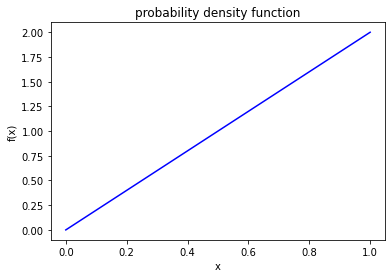
\includegraphics[width=\columnwidth]{assign2.png}
    \caption{Probability Density Function (PDF) of X}
    \label{Figure_1}
\end{figure}
The graph of PDF of X is \ref{Figure_1}
\par Let $F_X(x)$ be the cumulative distribution function of random variable X.
\begin{align}
    F_X(x)=\int_{-\infty}^x \fn{x} dx\label{x}
\end{align}
$F_X(x)$ can be obtained from the uniform distribution of a random variable U on (0,1) and let U=$X^2$. 
\begin{align}
    0 < U < 1
\end{align}
As for random variable X also,
\begin{align}
    0 < F_X(x) < 1
\end{align}
This similarity between U and $F_X(x)$ is used to generate the random variable X from U.
\begin{align}
    F_X(x)&= \pr{X<x}\\
    &=\pr{\sqrt{U}<x}\\
    &=\pr{U<x^2}\\
    &=F_U(x^2)\label{y}
\end{align}
From uniform distribution,
\\The graph of Probability Density Function (PDF) of U is \ref{Figure_2}
\begin{figure}[ht]
    \centering
    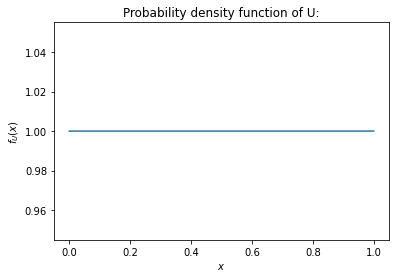
\includegraphics[width=\columnwidth]{assign2_2.png}
    \caption{Probability Density Function (PDF) of U}
    \label{Figure_2}
\end{figure}
\begin{align}
    F_U(x)=
    \begin{cases}
0 & x\leq0\\
x & 0<x<1
\\
1 & x\geq1\label{z}\\
\end{cases}
\end{align}
\begin{figure}[ht]
    \centering
    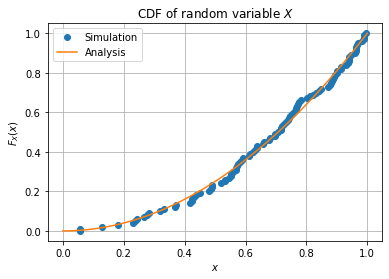
\includegraphics[width=\columnwidth]{assign2_1.png}
    \caption{Cumulative Density Function (CDF)}
    \label{Figure_3}
\end{figure}
\\Using \eqref{z} in \eqref{y},
\\Cumulative distribution function (CDF) of random variable X is,
\begin{align}
F_X(x)= \pr{X<x}
= 
\begin{cases}
0 & x\leq0\\
x^2 & 0<x<1
\\
1 & x\geq1\label{g}\\
\end{cases}
\end{align}
The graph of Cumulative distribution function (CDF) of random variable X is \ref{Figure_3}\\
Now we have to find \pr{X<0.5},Using  \eqref{g},
\begin{align}
    \pr{X<0.5} &= (0.5)^2\\
  \implies \pr{X<0.5} &= 0.25
\end{align}
\end{document}
